\documentclass{article}
\usepackage{graphicx}
\usepackage{amsmath}
\usepackage{float}
\usepackage{polski}
\usepackage[utf8]{inputenc}
\usepackage{mathtools}
\usepackage{caption}
\captionsetup{justification   = raggedright,
              singlelinecheck = false}

\title{Najlepszy Dziekan}
\date{Styczeń 2021}

\begin{document}
%\maketitle
\section{Niecodzienne spotkanie}
\indent Nie uwierzycie co mi się dzisiaj przydarzyło. Chodzę sobie jak zwykle po Wydziale, szukam dystrybutora z wodą, no i przechodzę przez łącznik, w nim piździ jak zwykle, środek zimy. I chce mi się kichnąć, kicham, a tu przez te dziury między piętrami po bokach, po szybie ześlizguje się Dziekan Turzyński i celuje we mnie jakimś dziwnym pistoletem, takim jak te śmieszne termometry co się przykłada do głowy. Ja w szoku, patrzę na podłogę, a tu żadnych śladów mojego kichnięcia! No ale ładnie się witam, dzień dobry Panie Dziekanie, pytam co to za zaszczyt że taka osobistość we mnie celuje. On na to, że to jego świeżo skonstruowany kwantowy wychwytywacz wirusa. No ale ja że Szanowny Panie Dziekanie, to nie lepiej się szczepić? A on że może tak, ale w tym chorym kraju nie da się żyć i że dopóki wszyscy się nie zaszczepią to on będzie tego wirusa wychwytywał. Potem wirus tuneluje przez Banacha i trafia na WUM, gdzie Dziekan korzysta z nieograniczonych możliwości swojej prawej ręki, bierze wirusa i go spala. Lekarze mu tam opatrują rękę itd. a on potem wraca na Wydział bo właśnie ma dyżur zdalnego Dziekana. I mówi że robi to wszystko z niepohamowanej miłości do studentów, żebyśmy wszyscy mieli stacjo bo on martwi się naszym zdrowiem psychicznym i rachunkami za Internet bo wiadomo jak jest. \\
\indent W ogóle wtedy oświeciło mnie i wpadłem na pomysł rozwiązania bardzo trudnego problemu który badam i szybko na chusteczce do nosa którą wyciągnałem przed kichnięciem zapisałem zależność daną równaniem:
\begin{equation}
    dz\times ie^{ka}\hat{n}<3\cdot \mathcal{L}(\mathcal{O}(\Vec{v}\wedge \Vec{E})),
    \label{Eq1}
\end{equation}
gdzie wszystkie potrzebne jednostki położyłem jako 1.\\	
\indent Wracając do tematu, bardzo podziękowałem Dziekanowi za wszystkie jego wysiłki i powiedziałem że do zobaczenia, bo zaraz sesja i wiadomo Dziekan może się przydać. On jeszcze na odchodne pyta czy nie znam jakiś studentów co mają sprawy do załatwienia, bo chętnie podpisałby jakieś podanie do Dziekana o cokolwiek. Ja na to że nie, bo wszyscy moi znajomi pracują już w IT i zostałem tu sam, ale jak kogoś poznam to przekażę. Pewnie byście mi nie uwierzyli, zatem poniżej Rysunek 1 przedstawia Dziekana podczas procesu dezintegracji wirusa.
\flushleft
\begin{figure}[!h]
\centering
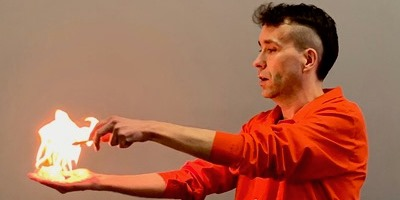
\includegraphics[width=.6\textwidth]{dziekan.jpg}
\caption{Najlepszy Dziekan.}
\label{dziekan}
\end{figure}


\end{document}
